\documentclass[tikz]{standalone}
\usepackage{tikz}
\usetikzlibrary{shapes.geometric, arrows}

\tikzstyle{startstop} = [rectangle, rounded corners, minimum width=3cm, minimum height=1cm, text centered, draw=black, fill=red!30]
\tikzstyle{process} = [rectangle, minimum width=3cm, minimum height=1cm, text centered, draw=black, fill=orange!30]
\tikzstyle{decision} = [diamond, minimum width=3cm, minimum height=1cm, text centered, draw=black, fill=yellow!30]
\tikzstyle{arrow} = [thick,->,>=stealth]

\begin{document}

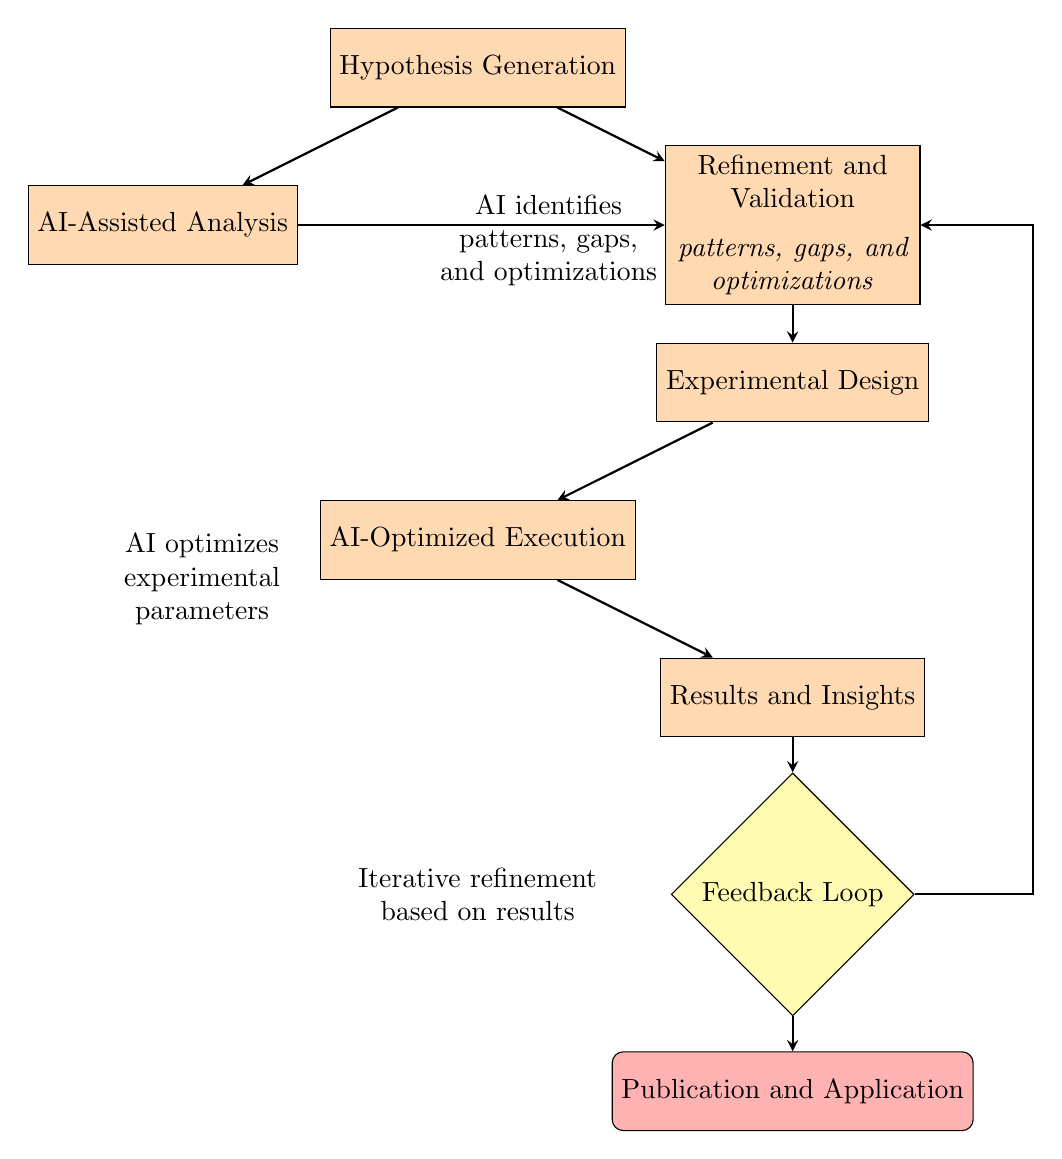
\begin{tikzpicture}[node distance=2cm]

    % Nodes
    \node (hypothesis) [process] {Hypothesis Generation};
    \node (ai1) [process, below of=hypothesis, xshift=-4cm] {AI-Assisted Analysis};
    \node (refinement) [process, below of=hypothesis, xshift=4cm] {
        \begin{minipage}{3cm}
            \centering
            Refinement and Validation \\
            \vspace{0.2cm}
            \textit{patterns, gaps, and optimizations}
        \end{minipage}
    };
    \node (experiment) [process, below of=refinement] {Experimental Design};
    \node (ai2) [process, below of=experiment, xshift=-4cm] {AI-Optimized Execution};
    \node (results) [process, below of=ai2, xshift=4cm] {Results and Insights};
    \node (feedback) [decision, below of=results, yshift=-0.5cm] {Feedback Loop};
    \node (publication) [startstop, below of=feedback, yshift=-0.5cm] {Publication and Application};

    % Arrows
    \draw [arrow] (hypothesis) -- (ai1);
    \draw [arrow] (hypothesis) -- (refinement);
    \draw [arrow] (ai1) -- (refinement);
    \draw [arrow] (refinement) -- (experiment);
    \draw [arrow] (experiment) -- (ai2);
    \draw [arrow] (ai2) -- (results);
    \draw [arrow] (results) -- (feedback);
    \draw [arrow] (feedback.east) -- ++(1.5,0) |- (refinement.east);
    \draw [arrow] (feedback) -- (publication);

    % Labels
    \node at (0.9,-2.2) [text width=3cm, align=center] {AI identifies patterns, gaps, and optimizations};
    \node at (-3.5,-6.5) [text width=3cm, align=center] {AI optimizes experimental parameters};
    \node at (0,-10.5) [text width=4cm, align=center] {Iterative refinement based on results};

\end{tikzpicture}

\end{document}
